\documentclass[a4paper, 12pt, oneside, onecolumn]{article}
\usepackage[utf8]{inputenc}
\usepackage[english]{babel}
\usepackage{geometry}
\usepackage{float}
\usepackage{graphicx}
\usepackage{amsmath}
\usepackage{amssymb}
\usepackage{systeme}
\usepackage{enumitem}
\usepackage{booktabs}
\usepackage{gensymb}
\usepackage{indentfirst}
\usepackage{bigints}
\usepackage{esint}
\usepackage{harpoon}
\usepackage{relsize}
\usepackage{cite}
\usepackage{url}
\usepackage{bm}
\usepackage{multicol}
\usepackage[useregional]{datetime2}
\usepackage[colorlinks = true, linkcolor = blue, hypertexnames = true]{hyperref}
\hypersetup{
    colorlinks=true,
    allcolors=blue	
}
\usepackage[super, square]{natbib}
\usepackage{lipsum}

\usepackage{epstopdf}
\usepackage{subfig}
\usepackage[subfigure]{tocloft}

\usepackage{authblk}


\newcommand{\cald}{{\rm d}}
\renewcommand\thesection{\Roman{section}}
\renewcommand{\thesubsection}{\thesection.\Roman{subsection}}
\renewcommand{\thesubsubsection}{\thesubsection.\Roman{subsubsection}}

\geometry{a4paper, scale = 0.85}
\linespread{1.5}

\setlength{\parindent}{2em}


\title{Mapping the Dance of the Stars:\\Unveiling the Dynamics of N-Body Simulations}

\author[$^\dagger$]{Gauss T. Chang}
\affil[$^\dagger$]{\textit{Department of Physics, National Taiwan University, Taipei, Taiwan}\\\texttt{b09501028@ntu.edu.tw}}



\date{\DTMdate{2024-12-17}}


\begin{document}
\maketitle

\begin{abstract}
	The N-body problem lies at the heart of understanding complex gravitational interactions, from planetary systems to galactic dynamics. This article explores the computational approach to solving the N-body problem, leveraging the power of Fortran for efficient simulation. I analyze the evolution of the system's energy and angular momentum to ensure conservation laws are upheld, a crucial benchmark for the accuracy of numerical methods. Additionally, statistical analyses provide insights into the emergent behaviors and stability of the system, further illustrating the robustness of the simulation.

	This work sheds light on how N-body simulations continue to transform our understanding of the cosmos, offering a gateway to unraveling the mysteries of celestial mechanics.
\end{abstract}
\begin{multicols}{2}


\section{Introduction}

The $N$-body problem, which seeks to determine the motions of $N$ distinct masses under mutual gravitational influence, has long been central to our understanding of celestial mechanics and astrophysical systems. While closed-form solutions are limited to special cases, computational simulations now serve as essential tools for studying the evolution of complex systems such as star clusters, planetary systems, and galaxies.

Despite its importance, the $N$-body problem poses significant computational and numerical challenges. The complexity of direct pairwise force evaluations scales as $O(N^2)$, becoming prohibitively expensive for large $N$. Additionally, the need to maintain physical fidelity—such as conserving energy and angular momentum—demands careful selection of numerical integration methods and collision-handling procedures.

This article focuses on a computational approach that harnesses both the classical laws governing gravitational interaction and modern approximation techniques to accelerate computations. I implement and test a Barnes–Hut algorithm to reduce computational complexity to approximately $O(N \log N)$, and I monitor key invariants such as total energy and angular momentum to assess the quality of the simulation. Furthermore, I explore performance improvements and discuss approaches to scaling these methods to larger systems.

In the following sections, I detail the theoretical foundations and algorithms employed (Section~\ref{sec:algorithm}), describe the simulation setup (Section~\ref{sec:Simulation-Setup}), present the results, and evaluate the performance and fidelity of my approach.


\section{Algorithm}\label{sec:algorithm}

In order to model the gravitational interactions among $N$ bodies, I start from fundamental physical laws and incorporate efficient computational techniques. This section first reviews Newton’s Law of Gravitation, the force model at the core of my simulation, and then introduces the Barnes–Hut algorithm, which significantly reduces the computational burden for large $N$.

\subsection{Newton’s Law of Gravitation}

The gravitational force between two point masses $m_1$ and $m_2$ separated by a distance vector $\mathbf{r} = \mathbf{r}_1 - \mathbf{r}_2$ is given by
\begin{equation}
\mathbf{F} = -G \frac{m_1 m_2}{|\mathbf{r}|^3} \mathbf{r},
\end{equation}
where $G$ is the gravitational constant. This force is attractive and acts along the line connecting the two masses. In an $N$-body system, each particle experiences forces from every other particle, leading to a set of coupled, nonlinear ordinary differential equations. For large $N$, evaluating each pairwise force directly leads to an $O(N^2)$ complexity, a severe limitation for computational studies of large-scale structures.

To handle dynamical evolution, we employ numerical integration methods. In this study, we utilize time-stepping integrators that update particle velocities and positions incrementally. Ensuring that these integrators preserve essential physical invariants, such as total energy and angular momentum, is key to obtaining meaningful and stable long-term results.

\subsection{Barnes–Hut Algorithm\cite{barnes_hierarchical_1986}}

The Barnes–Hut algorithm addresses the scaling issue inherent in direct $N$-body simulations. Rather than evaluating every particle-particle interaction, the algorithm builds a hierarchical tree structure to group particles that are sufficiently distant into a single effective mass at their combined center of mass. By treating distant clusters of particles as single entities, the force calculation for a given particle becomes more efficient, reducing the typical complexity to $O(N \log N)$.

The core idea is to recursively subdivide the computational domain into cells (quadrants in 2D or octants in 3D), constructing a tree that represents the spatial distribution of particles. Each internal node of the tree corresponds to a cell containing a group of particles, characterized by their total mass and center of mass. During the force calculation phase, if a node is sufficiently far away relative to its size, it can be used as a single approximation source. Otherwise, the tree is traversed further down to obtain finer-grained information.

By carefully tuning parameters such as the opening angle $\theta$, one can achieve a balance between accuracy and performance. A smaller $\theta$ yields more accurate results at the cost of additional computations, whereas a larger $\theta$ trades off accuracy for speed.





\subsection{Time Integration}

In this work, we start with a simple Euler method for time integration. For each particle, given a timestep $\Delta t$:

\begin{align}
	\mathbf{x}(t + \Delta t)
	&= \mathbf{x}(t) + \mathbf{\dot{x}}(t) \cdot \Delta t \\
	\mathbf{\dot{x}}(t + \Delta t)
	&= \mathbf{\dot{x}}(t) + \mathbf{\ddot{x}}(t) \cdot \Delta t
\end{align}

However, the Euler method, while straightforward, is only first-order accurate in $\Delta t$ and can lead to significant energy drift over long timescales. To improve accuracy and better conserve physical invariants such as total energy and angular momentum, we incorporate higher-order integration schemes derived from the Taylor expansion of position and velocity at $t + \Delta t$:

\begin{align}
	\mathbf{x_1} \nonumber
	&= \mathbf{x_0} + \frac{1}{2}\left(\mathbf{\dot{x}_0} + \mathbf{\dot{x}_1}\right)\Delta t \\
	&+ \frac{1}{12}\left(\mathbf{a_0} - \mathbf{a_1}\right)\Delta t^2+ O\left(\Delta t^5\right) \\
	\mathbf{\dot{x}_1} \nonumber
	&= \mathbf{\dot{x}_0} + \frac{1}{2}\left(\mathbf{a_0} + \mathbf{a_1}\right)\Delta t \\
	&+ \frac{1}{12}\left(\mathbf{\dot{a}_0} - \mathbf{\dot{a}_1}\right)\Delta t^2 + O\left(\Delta t^5\right)
\end{align}

Such higher-order and symplectic integrators (e.g., velocity Verlet) provide better long-term stability and minimize numerical artifacts that arise from approximation errors. In future enhancements, we may employ adaptive timestepping or even more sophisticated integrators to robustly handle close encounters, large $N$ systems, and complex dynamical scenarios.




\subsection{Elastic Collision}

In my simulation, particles are modeled as spherical masses that can collide elastically. A collision occurs when the distance between two particles $a$ and $b$ is less than or equal to the sum of their radii:
\begin{align}
	\left|\mathbf{x}_a - \mathbf{x}_b \right|
	& \leq \left( r_a + r_b \right)
\end{align}

Once a collision is detected, we resolve it by treating the encounter as a one-dimensional elastic collision along the line connecting the particle centers. Define the unit normal vector:
\begin{align}
	\mathbf{n}
	&= \frac{\mathbf{x}_a - \mathbf{x}_b}{\left|\mathbf{x}_a - \mathbf{x}_b\right|}
\end{align}

The relative velocity of the particles along this normal direction is: \begin{equation} v_{\text{rel}, n} = \left(\mathbf{v}_a - \mathbf{v}_b\right) \cdot \mathbf{n}. \end{equation}

If $v_{\text{rel}, n}$ is positive, the particles are already moving apart, and no collision response is needed. Otherwise, we compute an impulse $J$ that, when applied equally and oppositely to the two particles, conserves both momentum and kinetic energy. For masses $m_a$ and $m_b$, the magnitude of the impulse is: \begin{equation} J = \frac{2,v_{\text{rel}, n}}{\frac{1}{m_a} + \frac{1}{m_b}}. \end{equation}

The post-collision velocities are then updated as follows: \begin{align} \mathbf{v}_a' &= \mathbf{v}_a - \frac{J}{m_a}\mathbf{n}, \ \mathbf{v}_b' &= \mathbf{v}_b + \frac{J}{m_b}\mathbf{n}. \end{align}

This formulation ensures that the collision is perfectly elastic. Kinetic energy and linear momentum along the collision line are conserved, and the particles no longer overlap following the collision response. Such a treatment, while idealized, is sufficient for maintaining physically consistent behavior in the simulated system and preventing unrealistic particle interpenetrations.


\section{Simulation Setup}\label{sec:Simulation-Setup}

For my simulations, we begin by generating an initial distribution of $N$ particles placed within a cubic volume of side length $L$. Each particle is assigned:

\begin{itemize}
    \item \textbf{Mass:} Chosen randomly between $1$ and $2$, ensuring a modest mass contrast.
    \item \textbf{Position:} Initialized from a uniform distribution within the domain $$-\frac{L}{2}  \leq x, y, z \leq \frac{L}{2} $$
    \item \textbf{Velocity:} Drawn from a small uniform range (e.g., $-1$ to $1$), providing a non-zero initial kinetic state that allows the system to evolve dynamically.
    \item \textbf{Radius:} Assigned between $0.001$ and $0.05$, enabling detection and handling of elastic collisions when particles come into close proximity.
\end{itemize}

These initial conditions, as illustrated in the project slides, serve as a simple yet flexible baseline for exploring gravitational dynamics. The time domain is discretized into steps of size $\Delta t$. At each timestep, we:

\begin{enumerate}
    \item \textbf{Build the Barnes--Hut tree:} Particles are sorted into a hierarchical structure for efficient force approximations.
    \item \textbf{Compute Forces:} Gravitational forces on each particle are derived using the Barnes--Hut approximation. Close pairs are treated at a finer resolution, while distant groups of particles are represented by their center of mass.
    \item \textbf{Handle Collisions:} If two particles overlap (based on their radii), we resolve their encounter with an elastic collision model, preserving linear momentum and ensuring a physically plausible outcome.
    \item \textbf{Update Kinematics:} Particle positions and velocities are integrated forward in time using a chosen time integrator. We record total energy and angular momentum after each update to monitor numerical fidelity.
\end{enumerate}

By proceeding in this manner, we can visualize the initial random configurations evolving into complex structures, as demonstrated in my slide presentations and supplementary animations. These setups, while simplified, are an effective proving ground for testing algorithmic performance, verifying energy and momentum conservation, and identifying numerical drift in large-$N$ simulations.


\end{multicols}


\section{Results}

\subsection{Angular Momentum}

\begin{figure}[H]
	\centering
	\subfloat[Angular momentum v.s. time, $N = 32$ \label{AM32}]{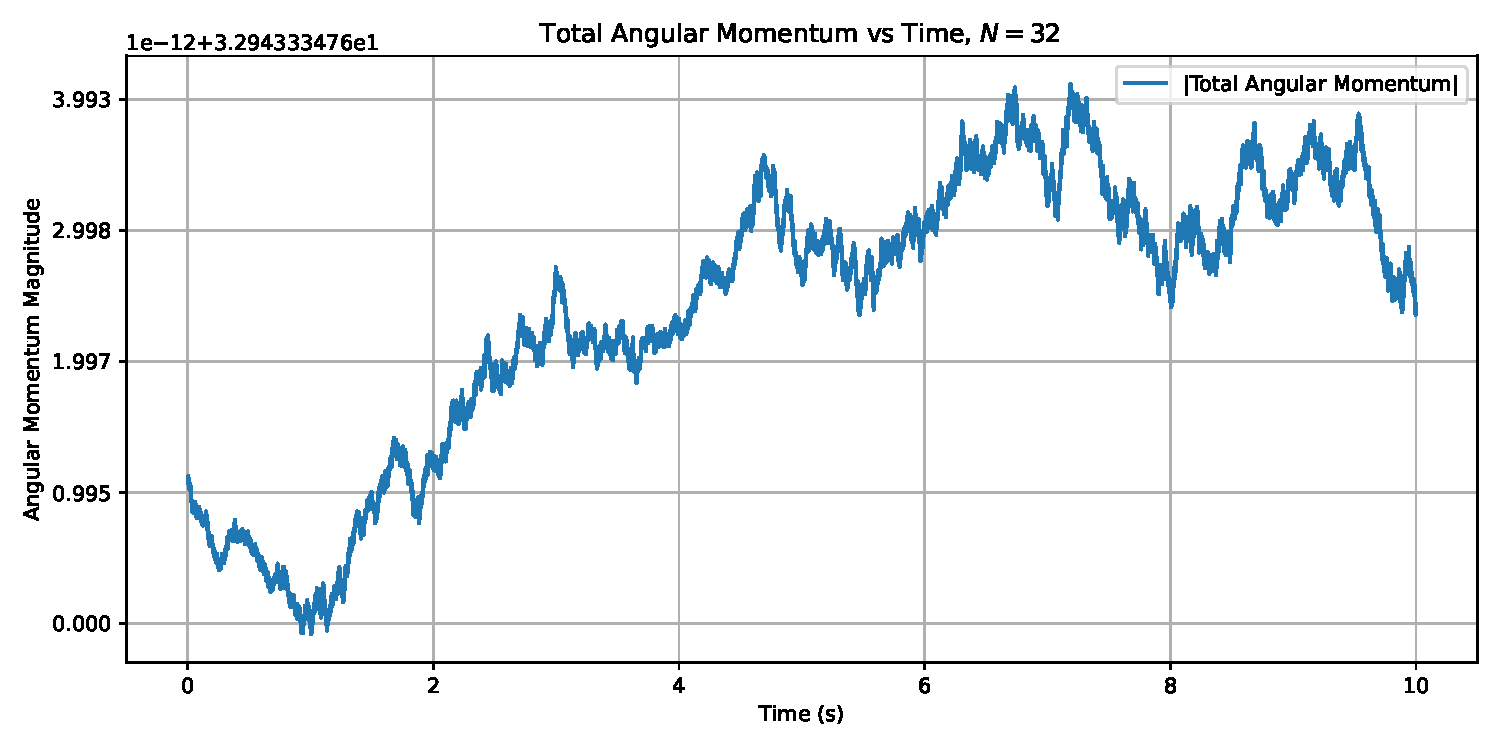
\includegraphics[width=.45\columnwidth]{../plot/cc_angular_momentum_vs_time_32_points.pdf}} \hspace{5pt}
	\subfloat[Angular momentum v.s. time, $N = 64$ \label{AM64}]{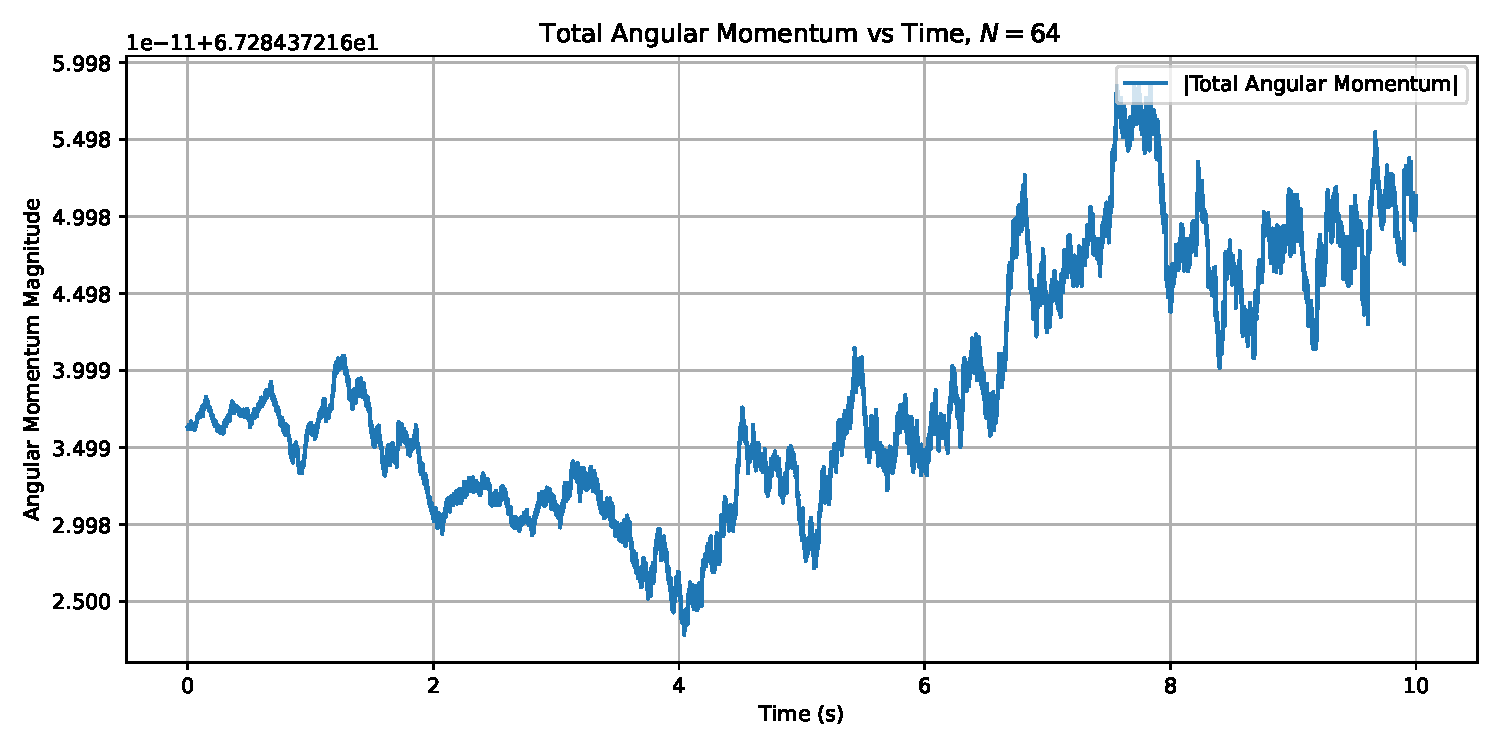
\includegraphics[width=.45\columnwidth]{../plot/cc_angular_momentum_vs_time_64_points.pdf}} \\
	\subfloat[Angular momentum v.s. time, $N = 128$ \label{AM128}]{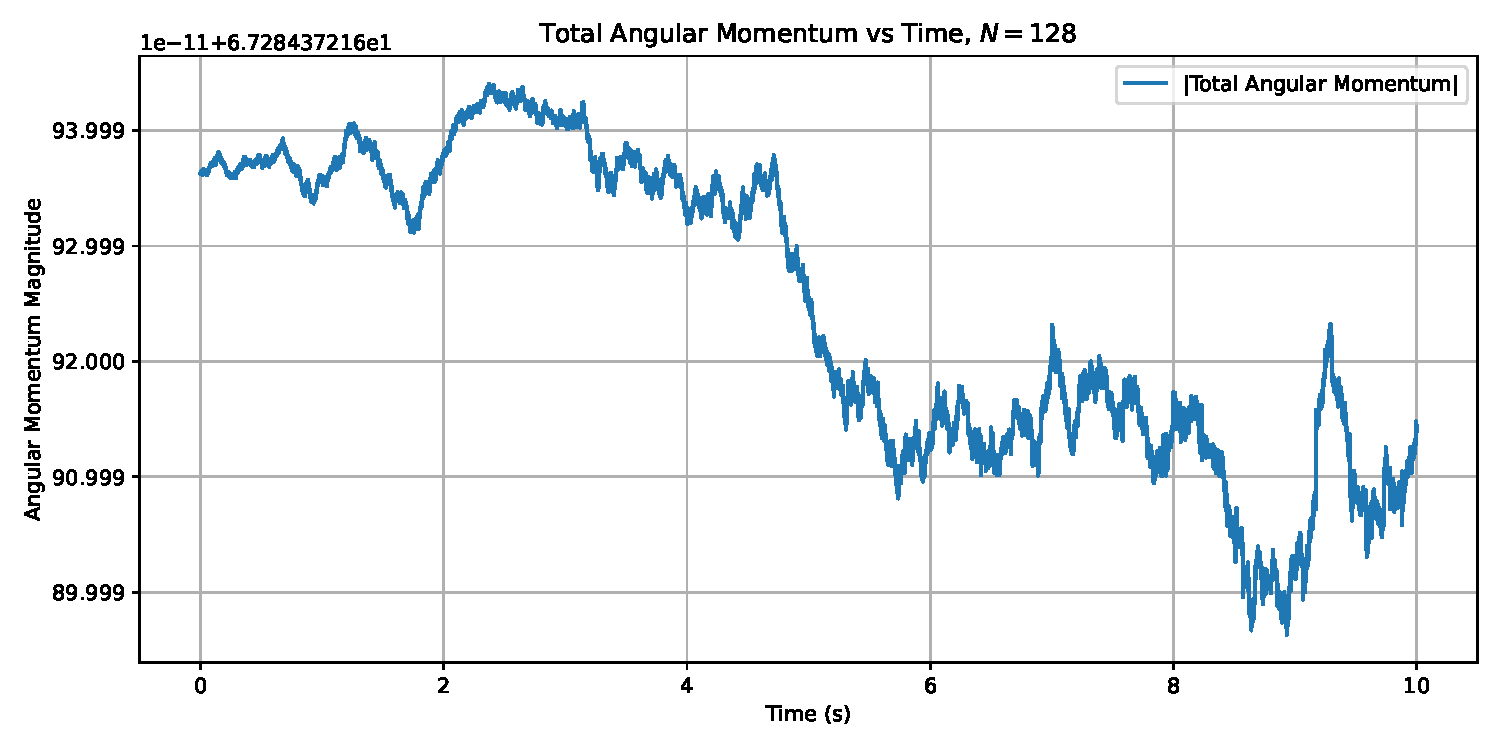
\includegraphics[width=.45\columnwidth]{../plot/cc_angular_momentum_vs_time_128_points.pdf}} \hspace{5pt}
	\subfloat[Angular momentum v.s. time, $N = 256$ \label{AM256}]{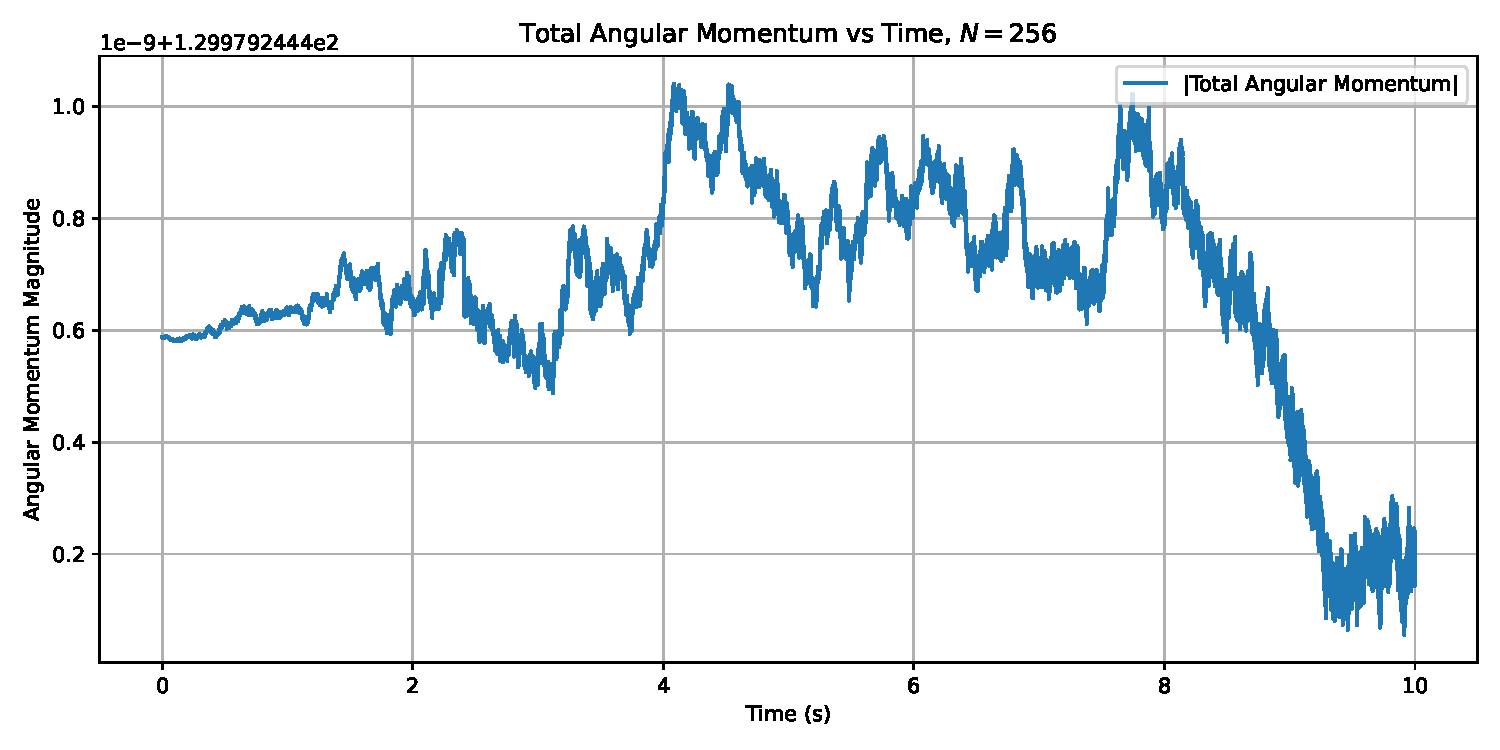
\includegraphics[width=.45\columnwidth]{../plot/cc_angular_momentum_vs_time_256_points.pdf}} \\
	\caption{Angular momentum v.s. time for different particle number.}
\end{figure}

\begin{multicols}{2}

Angular momentum is a critical conserved quantity in gravitational systems, reflecting the rotational invariants of the system’s motion. In principle, a well-posed $N$-body simulation with accurate numerical integration and appropriate timestep selection should preserve total angular momentum over time.

Figures~\ref{AM32}--\ref{AM256} show the evolution of the total angular momentum magnitude as a function of time for simulations with $N = 32, 64, 128,$ and $256$ particles. Overall, the angular momentum remains remarkably stable throughout the simulations. Although minor fluctuations are present, it is important to consider them in the context of the scale of the system’s total angular momentum.

Our simulations maintain a total angular momentum on the order of $10^1$, and the observed fluctuations are on the order of $10^{-9}$ to $10^{-11}$. In other words, the relative change in angular momentum is extremely small, on the order of $10^{-10}$ relative to the magnitude of the total angular momentum. Such tiny deviations are well within acceptable bounds for numerical simulations involving floating-point arithmetic and are likely attributable to truncation errors, round-off errors, and other numerical artifacts inherent in large-scale computations.

Unlike total energy, which can drift more significantly under certain conditions (especially at larger $N$ or after numerous collision events), angular momentum appears robust and shows no trend of systematic loss or gain over time. This stability suggests that our choice of integration scheme, timestep, and collision handling mechanism effectively preserves rotational invariants. Further refinement of the integration methods or employing adaptive time-stepping could reduce these minuscule fluctuations even more, but for the purposes of this study, the current level of angular momentum conservation is fully satisfactory.

In conclusion, the angular momentum results confirm that the numerical approach and algorithms implemented here are both stable and reliable, providing a solid foundation for exploring more complex gravitational systems.

\end{multicols}


\subsection{Total Energy}

\begin{figure}[H]
	\centering
	\subfloat[Total energy v.s. time, $N = 32$ \label{TE32}]{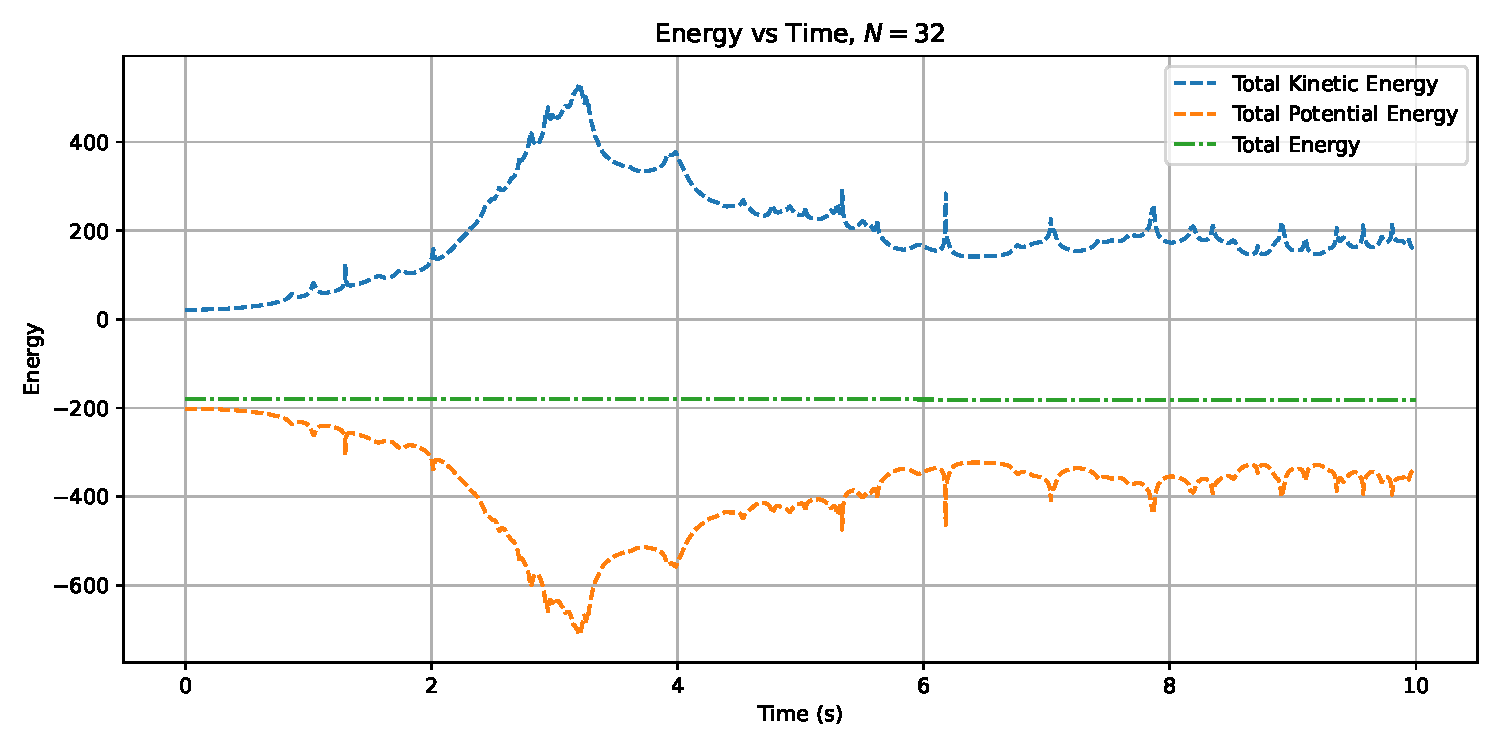
\includegraphics[width=.45\columnwidth]{../plot/cc_energy_vs_time_32_points.pdf}} \hspace{5pt}
	\subfloat[Total energy v.s. time, $N = 64$ \label{TE64}]{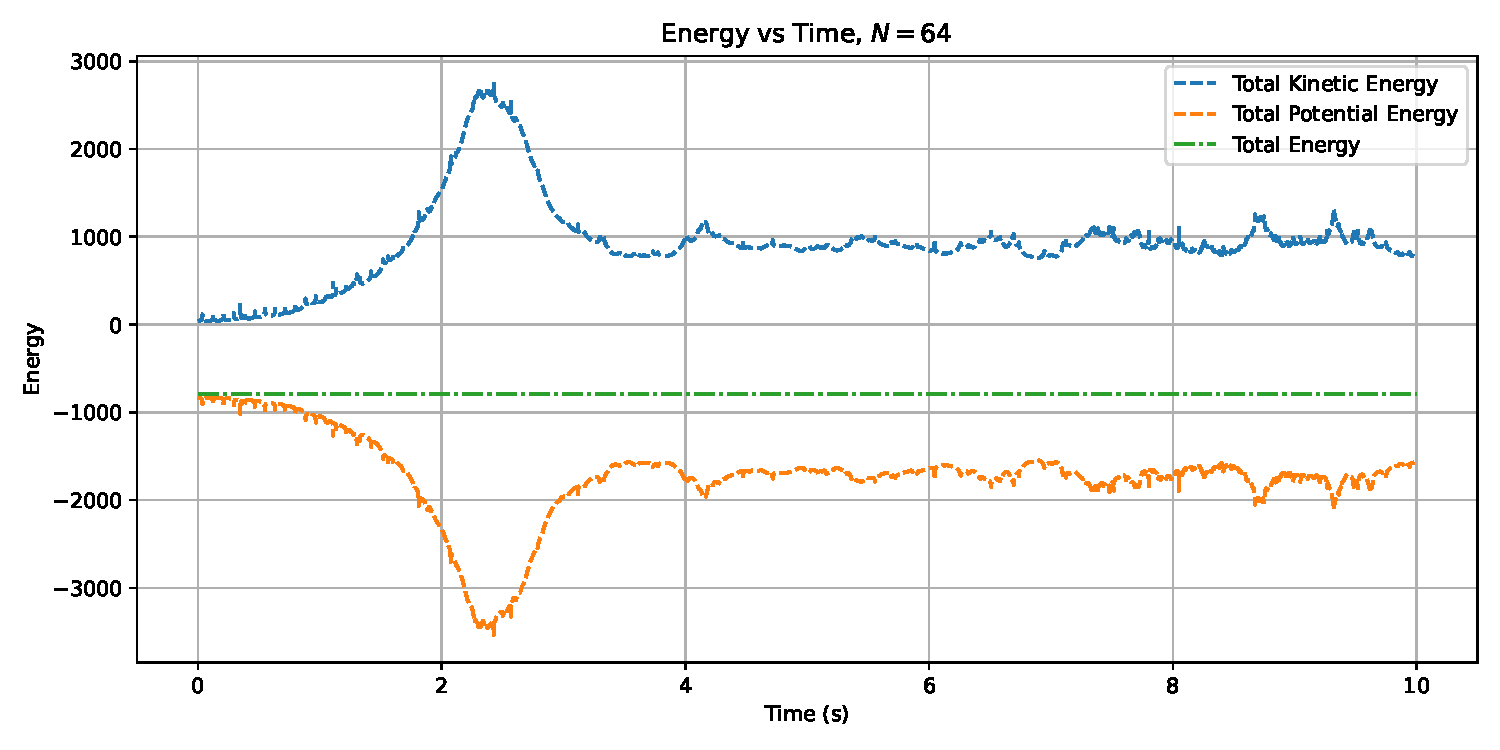
\includegraphics[width=.45\columnwidth]{../plot/cc_energy_vs_time_64_points.pdf}} \\
	\subfloat[Total energy v.s. time, $N = 128$ \label{TE128}]{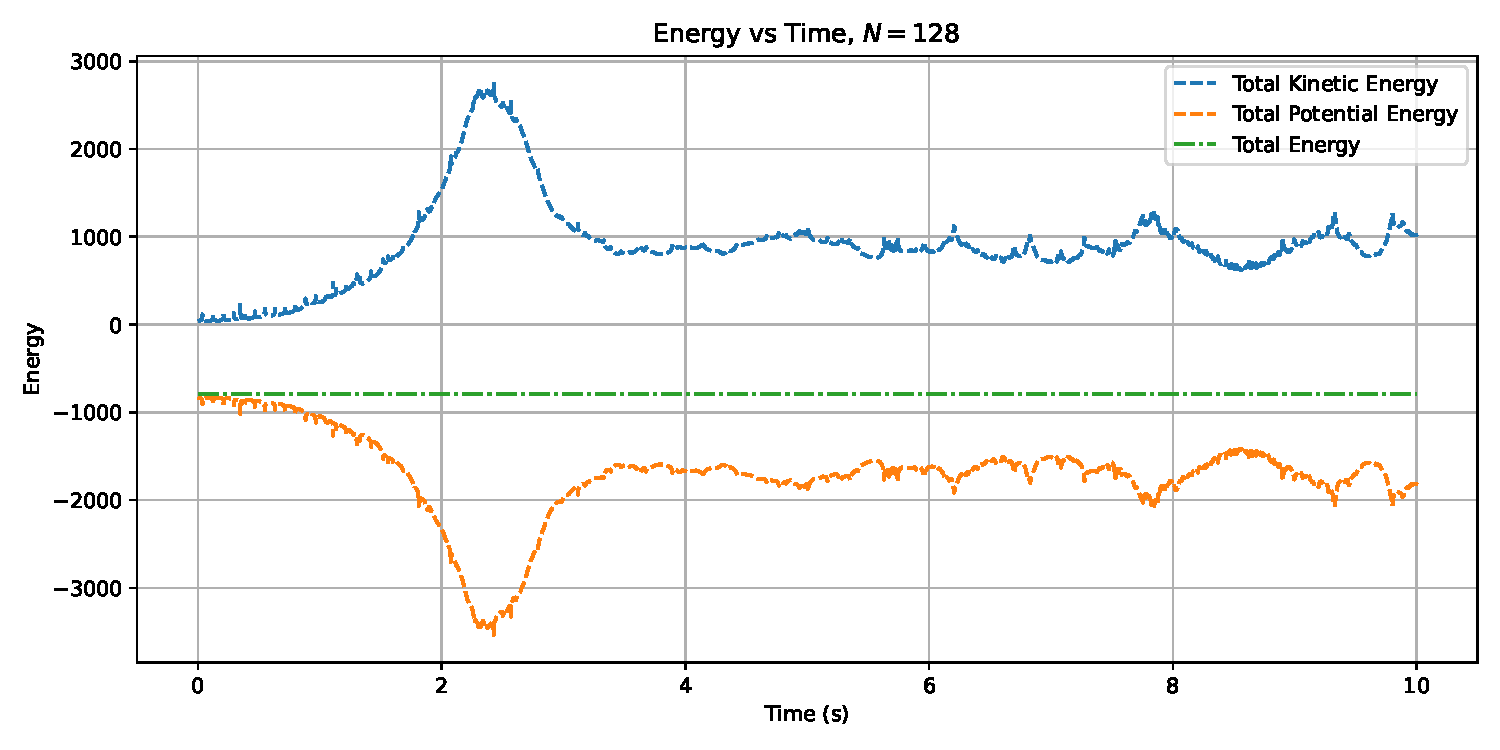
\includegraphics[width=.45\columnwidth]{../plot/cc_energy_vs_time_128_points.pdf}} \hspace{5pt}
	\subfloat[Total energy v.s. time, $N = 256$ \label{TE256}]{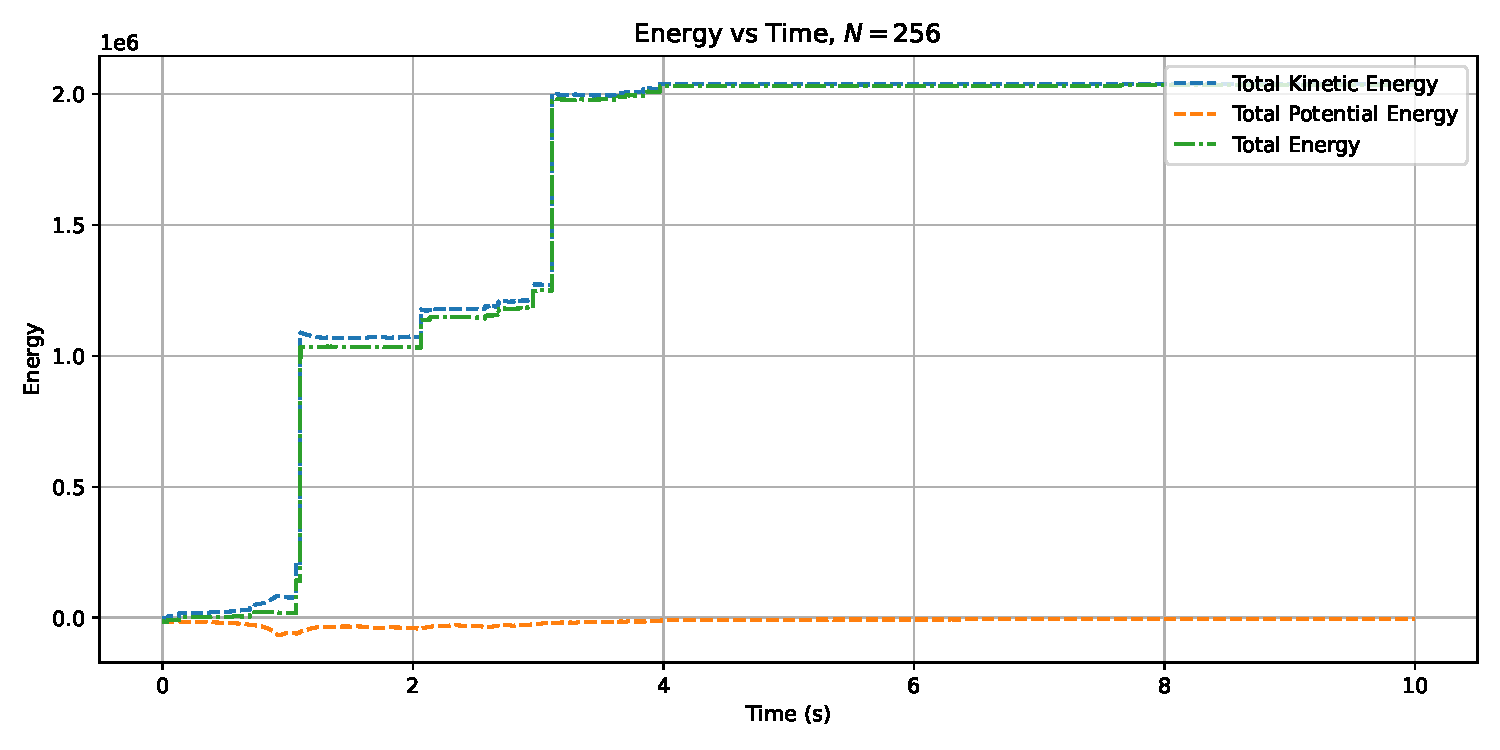
\includegraphics[width=.45\columnwidth]{../plot/cc_energy_vs_time_256_points.pdf}} \\
	\caption{Total energy v.s. time for different particle number.}
\end{figure}

\begin{multicols}{2}

Conservation of total energy, $E_{\text{total}} = E_{\text{kinetic}} + E_{\text{potential}}$, is a stringent test of the numerical fidelity of $N$-body simulations. In principle, the gravitational $N$-body system should conserve its total energy if integrated perfectly and if collisions are handled in a physically consistent manner. However, numerical approximations, finite timestep sizes, and the accumulation of round-off and truncation errors can introduce energy drift over the course of the simulation.

Figures~\ref{TE32}--\ref{TE256} compares total kinetic, potential, and total energy for $N = 32, 64, 128,$ and $256$. For the smaller systems ($N = 32$ and $N = 64$), the total energy remains relatively stable over time, with only modest fluctuations that do not significantly diverge from the initial values. This indicates that, for these system sizes, our chosen timestep and integration schemes effectively preserve total energy on the timescales examined.

As I increase $N$ to $128$, there begin to be more pronounced variability in total energy, though the system still appears to retain rough energy balance. The fluctuations can be attributed to the increasing complexity of gravitational interactions and more frequent close encounters. Nevertheless, the energy still does not exhibit a catastrophic drift away from its initial level.

At $N = 256$, however, energy conservation begins to break down more noticeably. Over time, the total energy curve drifts significantly, indicating that the numerical errors and collision-related adjustments accumulate faster than they can be mitigated. This behavior points toward the need for more robust integration methods, smaller timesteps, or improved collision handling as $N$ grows large. The rapidly evolving and increasingly crowded environment of a high-$N$ system challenges the stability of the current approach, causing greater deviations from exact energy conservation.

In summary, while total energy is reasonably well conserved for smaller systems, higher particle numbers lead to more substantial energy drift. Future improvements, such as adaptive timestep selection or higher-order symplectic integrators, may be necessary to maintain better energy conservation in large-scale $N$-body simulations.





%\section{Discussion}
\section{Discussion}

The results presented in this work highlight both the capabilities and the limitations of our current $N$-body simulation approach. By examining key physical invariants—particularly total angular momentum and total energy—we gain insights into the accuracy and stability of our chosen numerical methods.

\subsection*{Angular Momentum Conservation}

The angular momentum results confirm that, for a wide range of particle numbers ($N = 32$ to $256$), the system retains its rotational invariants with only minimal numerical drift. Angular momentum deviations remain on the order of $10^{-9}$ to $10^{-11}$, even though the total angular momentum itself is on the order of $10^1$. This minuscule relative error suggests that the core integration scheme and collision model effectively preserve rotational characteristics over the simulated timescales. The stability of angular momentum across increasing complexity and particle number is encouraging and points to the robustness of the underlying algorithms used to approximate gravitational forces and handle particle interactions.

\subsection*{Energy Conservation and Scaling Challenges}

In contrast, energy conservation proves more challenging as $N$ grows. For small systems ($N = 32$ and $N = 64$), total energy remains relatively stable, indicating that the simple integration scheme and chosen timestep sizes are adequate for these modest scales. As we move to $N = 128$, fluctuations in total energy become more pronounced, yet still manageable, reflecting the increasing complexity and frequency of gravitational interactions and close encounters.

However, by $N = 256$, the simulation struggles to maintain energy conservation. The significant drift observed in total energy suggests that numerical errors accumulate more rapidly in dense and dynamically active environments. Factors contributing to this drift include:

\begin{itemize}
    \item \textbf{Integration Method Limitations:} While straightforward integrators like the Euler or low-order schemes are easy to implement, they do not guarantee long-term conservation of energy. The cumulative effect of truncation errors becomes substantial as $N$ increases.
    \item \textbf{Collision Handling:} Although our elastic collision model conserves momentum and kinetic energy in the instantaneous interaction, multiple collisions and close encounters introduce subtle numerical artifacts. Over many timesteps, small inaccuracies can accumulate, contributing to observable energy drift.
    \item \textbf{Parameter Choices:} A fixed timestep $\Delta t$ may be appropriate for small $N$ but becomes less optimal for larger systems that contain regions of high density and rapidly changing gravitational potentials. Without adaptive refinement, large systems can rapidly develop unstable numerical behaviors.
\end{itemize}

\subsection*{Implications for Large-Scale Simulations}

The observed energy drift at higher $N$ highlights the need for more sophisticated integration strategies when scaling up simulations. Approaches such as symplectic integrators, velocity Verlet, or other higher-order methods can provide more accurate long-term energy conservation. Additionally, adaptive timestep selection—where smaller timesteps are used during close encounters or in dense regions—could mitigate some of the errors that accumulate in large, complex systems.

Beyond integration methods, data structures like the Barnes–Hut tree, which have already proven effective in reducing computational complexity, can be further optimized. More accurate cell-opening criteria or hybrid approaches that combine direct summation for near-neighbors with Barnes–Hut approximations for distant particles might yield improved stability.

Finally, considering that this study utilized relatively small particle numbers compared to state-of-the-art astrophysical simulations, these findings underscore the importance of careful algorithmic choices as I approach massively parallel, million- or billion-particle simulations. The lessons learned here—balancing accuracy, efficiency, and stability—are directly relevant to advancing the field of computational astrophysics, where precise $N$-body solvers underpin our understanding of gravitational clustering, galaxy formation, and large-scale cosmological structures.

\subsection*{Future Directions}

Moving forward, several improvements are possible:

\begin{itemize}
    \item \textbf{Higher-Order and Symplectic Integrators:} Implementing integrators designed to conserve phase-space volume and energy more rigorously over long timescales could yield more stable results, especially for large $N$.
    \item \textbf{Adaptive Timestepping:} Dynamically adjusting the timestep in response to the system’s local conditions would help resolve close encounters more accurately, reducing the accumulation of numerical errors.
    \item \textbf{Refined Collision Models:} Incorporating more physically realistic collision treatments or implementing methods that minimize unphysical overlapping states could improve overall energy stability.
    \item \textbf{Scaling Tests:} Testing larger $N$ systems, perhaps combined with GPU acceleration or parallel computing strategies, would provide valuable insight into how well these solutions scale and where bottlenecks occur.
\end{itemize}

In conclusion, while our simulations demonstrate stable angular momentum conservation and reliable energy behavior for smaller $N$, the results at higher $N$ emphasize the need for more advanced numerical techniques. By refining our integration schemes, timestepping strategies, and collision handling, I can push toward more accurate, stable, and scalable $N$-body simulations, ultimately gaining a deeper understanding of gravitational interactions in complex astrophysical environments.








\end{multicols}


%\newpage
\section*{Acknowledgments}
This is a final report for a course on the Computer Programming on Geosciences, written by a senior student from the Department of Physics at National Taiwan University. Please note that I have tried my best to eliminate typos and errors. So if there are any, they are unintentional, and I ask for your understanding and forgiveness.
\section*{Author Declarations}
\subsection*{Conflict of Interest}
The authors have no conflicts to disclose.
\newpage
\nocite{*}
\bibliographystyle{unsrt}
\bibliography{./bibliography.bib}
\end{document}








































